\begin{frame}
    \frametitle{Método}
    \framesubtitle{Interacción}

    \begin{columns}
        \begin{column}{0.3\textwidth}
            \begin{center}
                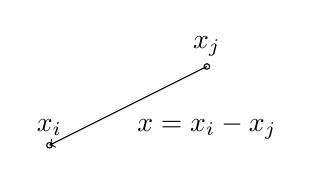
\begin{tikzpicture}
                    \draw (-1,-0.5) circle (1pt) node[above] {$x_{i}$};
                    \draw (1,0.5)   circle (1pt) node[above] {$x_{j}$};
                    \draw [<-] (-1,-0.5) -- (1,0.5) node[below=0.5cm] {$x = x_{i} - x_{j}$};
                \end{tikzpicture}
            \end{center}
        \end{column}
        \begin{column}{0.7\textwidth}
            \small
            \begin{eqnarray}
                \Phi_{i} &=& \sum_{j=0}^{N} \frac{m_{j}}{r} \\
                r &=& \sqrt{(x_{i}-x_{j})^2 + (y_{i}-y_{j})^2 + (z_{i}-z_{j})^2} \\
                  &=& \sqrt{x^{2} + y^{2} + z^{2}} \nonumber
            \end{eqnarray}
        \end{column}
    \end{columns}
\end{frame}

\begin{frame}
    \frametitle{Método}
    \framesubtitle{Conjunto de partículas}

    \begin{center}
        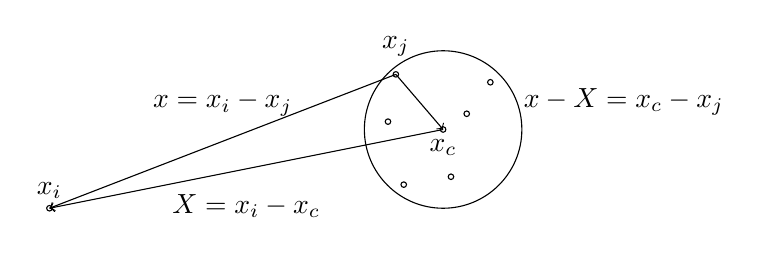
\begin{tikzpicture} 
            \draw (0,0)      circle (1cm)
                  (-5,-1)    circle (1pt)
                  (0,0)      circle (1pt)
                  (-0.6,0.7) circle (1pt)
                  (-0.7,0.1) circle (1pt)
                  (-0.5,-0.7) circle (1pt)
                  (0.1,-0.6) circle (1pt)
                  (0.3,0.2) circle (1pt)
                  (0.6,0.6) circle (1pt);
            \draw [<-] (-5,-1) -- node[above=0.2cm] {$x = x_{i} - x_{j}$} (-0.6,0.7) node[above=0.1cm] {$x_{j}$};
            \draw [<-] (-5,-1) node[above] {$x_{i}$} -- node[below=0.2cm] {$X = x_{i} - x_{c}$} (0,0) node[below] {$x_{c}$};
            \draw [<-] (0,0)   -- node[right=1.2cm] {$x - X = x_{c} - x_{j}$} (-0.6,0.7);
        \end{tikzpicture}
    \end{center}

    $$\Phi_{i} = \sum_{j=0}^{N} m_{j} f(x),\ \ f(x) = \frac{1}{r}$$

\end{frame}


\begin{frame}
    \frametitle{Método}
    \framesubtitle{Expansión de Taylor}

    $$f(x) = f(a) + \frac{f'(a)}{1!} (x-a)+\frac{f''(a)}{2!} (x-a)^{2} + \cdots$$
    $$f(x) = \sum_{n=0}^{\infty} \frac{f^{(n)}(a)}{n!} (x-a)^{n}$$
    
\end{frame}

\begin{frame}
    \frametitle{Método}
    \framesubtitle{Expansión de Taylor}
    \tiny
    $$R = \sqrt{X^{2} + Y^{2} + Z^{2}}$$

    \begin{equation}
    \begin{split}
    f(x) = \frac{1}{r} = \frac{1}{R} +& \frac{1}{1!} \left[ (x-X)\frac{\partial}{\partial X} \frac{1}{R} + (y-Y)\frac{\partial}{\partial Y} \frac{1}{R} +(z-Z)\frac{\partial}{\partial Z} \frac{1}{R} \right] \\
                                     +& \frac{2}{2!} \left[ (x-X)^{2}\frac{\partial^{2}}{\partial X \partial X} \frac{1}{R} + (y-Y)^{2}\frac{\partial^{2}}{\partial Y\partial Y} \frac{1}{R} +(z-Z)^{2}\frac{\partial^{2}}{\partial Z\partial Z} \frac{1}{R} \right. \nonumber \\
                                     +& \left.(x-X)(y-Y) \frac{\partial^{2}}{\partial X \partial Y} \frac{1}{R} + (y-Y)(z-Z)\frac{\partial^{2}}{\partial Y\partial Z} \frac{1}{R} + (z-Z)(x-X)\frac{\partial^{2}}{\partial Z \partial X} \frac{1}{R} \right]
    \end{split}
    \end{equation}
\end{frame}

\begin{frame}
    \frametitle{Método}
    \framesubtitle{Expansión de Taylor}
    \tiny
    $$R = \sqrt{X^{2} + Y^{2} + Z^{2}}$$

    \begin{equation}
    \begin{split}
    f(x) = \frac{1}{r} = \frac{1}{R} +& \frac{1}{1!} \left[ (x-X)\red{\frac{\partial}{\partial X} \frac{1}{R}} + (y-Y)\red{\frac{\partial}{\partial Y} \frac{1}{R}} +(z-Z)\red{\frac{\partial}{\partial Z} \frac{1}{R}} \right] \\
                                     +& \frac{2}{2!} \left[ (x-X)^{2}\red{\frac{\partial^{2}}{\partial X \partial X} \frac{1}{R}} + (y-Y)^{2}\red{\frac{\partial^{2}}{\partial Y\partial Y} \frac{1}{R}} +(z-Z)^{2}\red{\frac{\partial^{2}}{\partial Z\partial Z} \frac{1}{R}} \right. \nonumber \\
                                     +& \left.(x-X)(y-Y) \red{\frac{\partial^{2}}{\partial X \partial Y} \frac{1}{R}} + (y-Y)(z-Z)\red{\frac{\partial^{2}}{\partial Y\partial Z} \frac{1}{R}} + (z-Z)(x-X)\red{\frac{\partial^{2}}{\partial Z \partial X} \frac{1}{R}} \right]
    \end{split}
    \end{equation}
\end{frame}


\begin{frame}
    \frametitle{Método}
    \framesubtitle{Componentes Expansión de Taylor}

    \footnotesize
    \begin{eqnarray}
        \frac{\partial}{\partial X} \frac{1}{R} &=& -\frac{X}{R^{3}}\nonumber \\
        \frac{\partial^{2}}{\partial X\partial X} \frac{1}{R} &=& \frac{3X^{2}}{R^{5}} - \frac{1}{R^{3}} \nonumber\\
        \frac{\partial^{2}}{\partial X\partial Y} \frac{1}{R} &=& \frac{3XY}{R^{5}} \nonumber
    \end{eqnarray}
    \normalsize
    Se reemplaza en la ecuación anterior...
    

\end{frame}


\begin{frame}
    \frametitle{Método}
    \framesubtitle{Forma generalizada Expansión de Taylor}
    \footnotesize
    $$\frac{1}{r} = \sum_{n=0}^{p} \frac{1}{n!} (x-X)^{n}\frac{\partial^{(n)}}{\partial X} \frac{1}{R}$$
    \begin{itemize}
        \item $X = x_{i} - x_{c}$, independiente de $j$.
        \item $x - X = x_{c} - x_{j}$, independiente de $i$. 
    \end{itemize}
    \tiny
    \begin{eqnarray}
        \Phi_{i} &=& \sum_{j=0}^{N} \frac{m_{j}}{r} \nonumber \\
                 &=& \sum_{j=0}^{N} m_{j}\sum_{n=0}^{p} \frac{1}{n!}(x-X)^{n}\frac{\partial^{(n)}}{\partial X} \frac{1}{R} \nonumber \\
                 &=& \sum_{n=0}^{p} \sum_{j=0}^{N} m_{j}\frac{1}{n!}(x-X)^{n}\frac{\partial^{(n)}}{\partial X} \frac{1}{R} \nonumber \\
                 &=& \sum_{n=0}^{p} \frac{\partial^{(n)}}{\partial X} \frac{1}{R} \underbrace{\sum_{j=0}^{N} m_{j}\frac{1}{n!}(x-X)^{n}}_{\mbox{multipole}} \nonumber \\
    \end{eqnarray}
\end{frame}

\begin{frame}
    \frametitle{Método}
    \framesubtitle{Forma generalizada Expansión de Taylor}

    $$\Phi_{i} = \sum_{n=0}^{p} \frac{\partial^{(n)}}{\partial X} \frac{1}{R} \sum_{j=0}^{N} m_{j}\frac{1}{n!}(x-X)^{n} $$
    $$\frac{1}{R^{n+1}}\ \ \ \ \ \ (r-R)^{n}$$
    $$\left(\frac{r-R}{R}\right)^{n} < 1$$
    $$ |x - X| < |X|$$
    
\end{frame}


\begin{frame}
    \frametitle{Método}
    \framesubtitle{Estructuras base}

    \begin{eqnarray}
        monopole &=& \sum_{j=0}^{N} m_{j} \nonumber \\
        dipole  &=& \sum_{j=0}^{N} m_{j} x_{jc} \nonumber \\
        quadrapole   &=& \sum_{j=0}^{N} \frac{1}{2} m_{j} x^{2}_{jc} \nonumber 
    \end{eqnarray}

\end{frame}
